\section{Mediciones}

Para tener una primera aproximación para obtener la complejidad del algoritmo, graficamos los tiempos de ejecución
de nuestro algoritmo para los ejemplos provistos por la cátedra. Ver figura \ref{fig:tiempos_ejemplos}.

\begin{figure}[H]
    \centering
    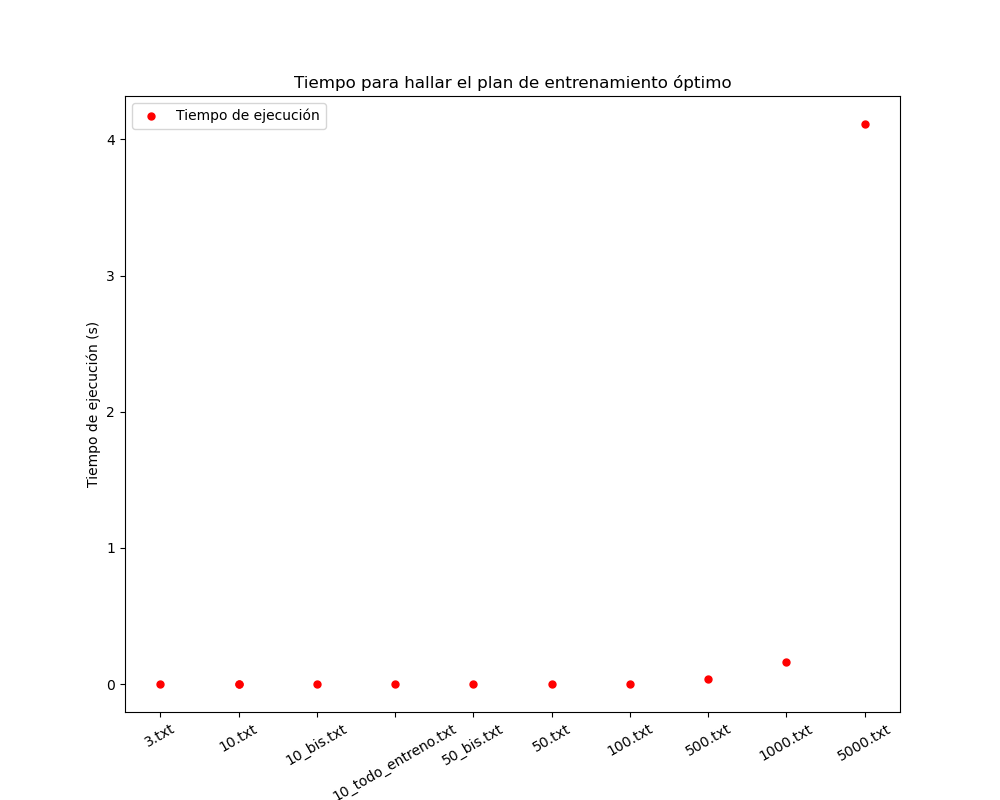
\includegraphics[width=0.8\textwidth]{img/tiempos_catedra.png}
    \caption{Tiempos de ejecución para los ejemplos provistos por la cátedra.}
    \label{fig:tiempos_ejemplos}
\end{figure}

A medida que aumenta el tamaño de la entrada, se observa un significativo incremento en el tiempo de ejecución.
Esto sugiere que la complejidad del algoritmo es considerablemente mayor que la lineal.

Para tener un gráfico de mediciones más determinístico, creamos escenarios de ejemplo de forma aleatoria. Cada escenario consta de
una lista de esfuerzos de cada día de entrenamiento y otra con las energías de cada día de
entrenamiento consecutivo. Decidimos que el los valores de esfuerzos y energías sean valor enteros
entre 1 y 99'999, basándonos en los datos de ejemplo provistos por la cátedra.

Medimos el tiempo de ejecución de nuestro algoritmo para ciertas cantidades de esfuerzos y energías.

Notamos que los procesos de fondo del sistema nos generaba distorciones en los tiempos de ejecución
de una misma muestra. Atacamos este problema realizando varias mediciones para el mismo escenario de
esfuerzos y energías, tomando el promedio de los tiempos obtenidos.

Con el objetivo de comparar los tiempos de ejecución de nuestro algoritmo con la complejidad teórica, optamos por 
realizar tanto un análisis de regresión cuadrática con una regresión exponencial que se ajustara a nuestros datos.
Para evaluar qué curva se ajusta mejor, usamos la raíz del error cuadrático medio (RMSE). Realizamos este análisis en un
intervalo con tamaños hasta 1'000. Ver figuras \ref{fig:tiempos_puntos}.

\begin{figure}[H]
    \centering
    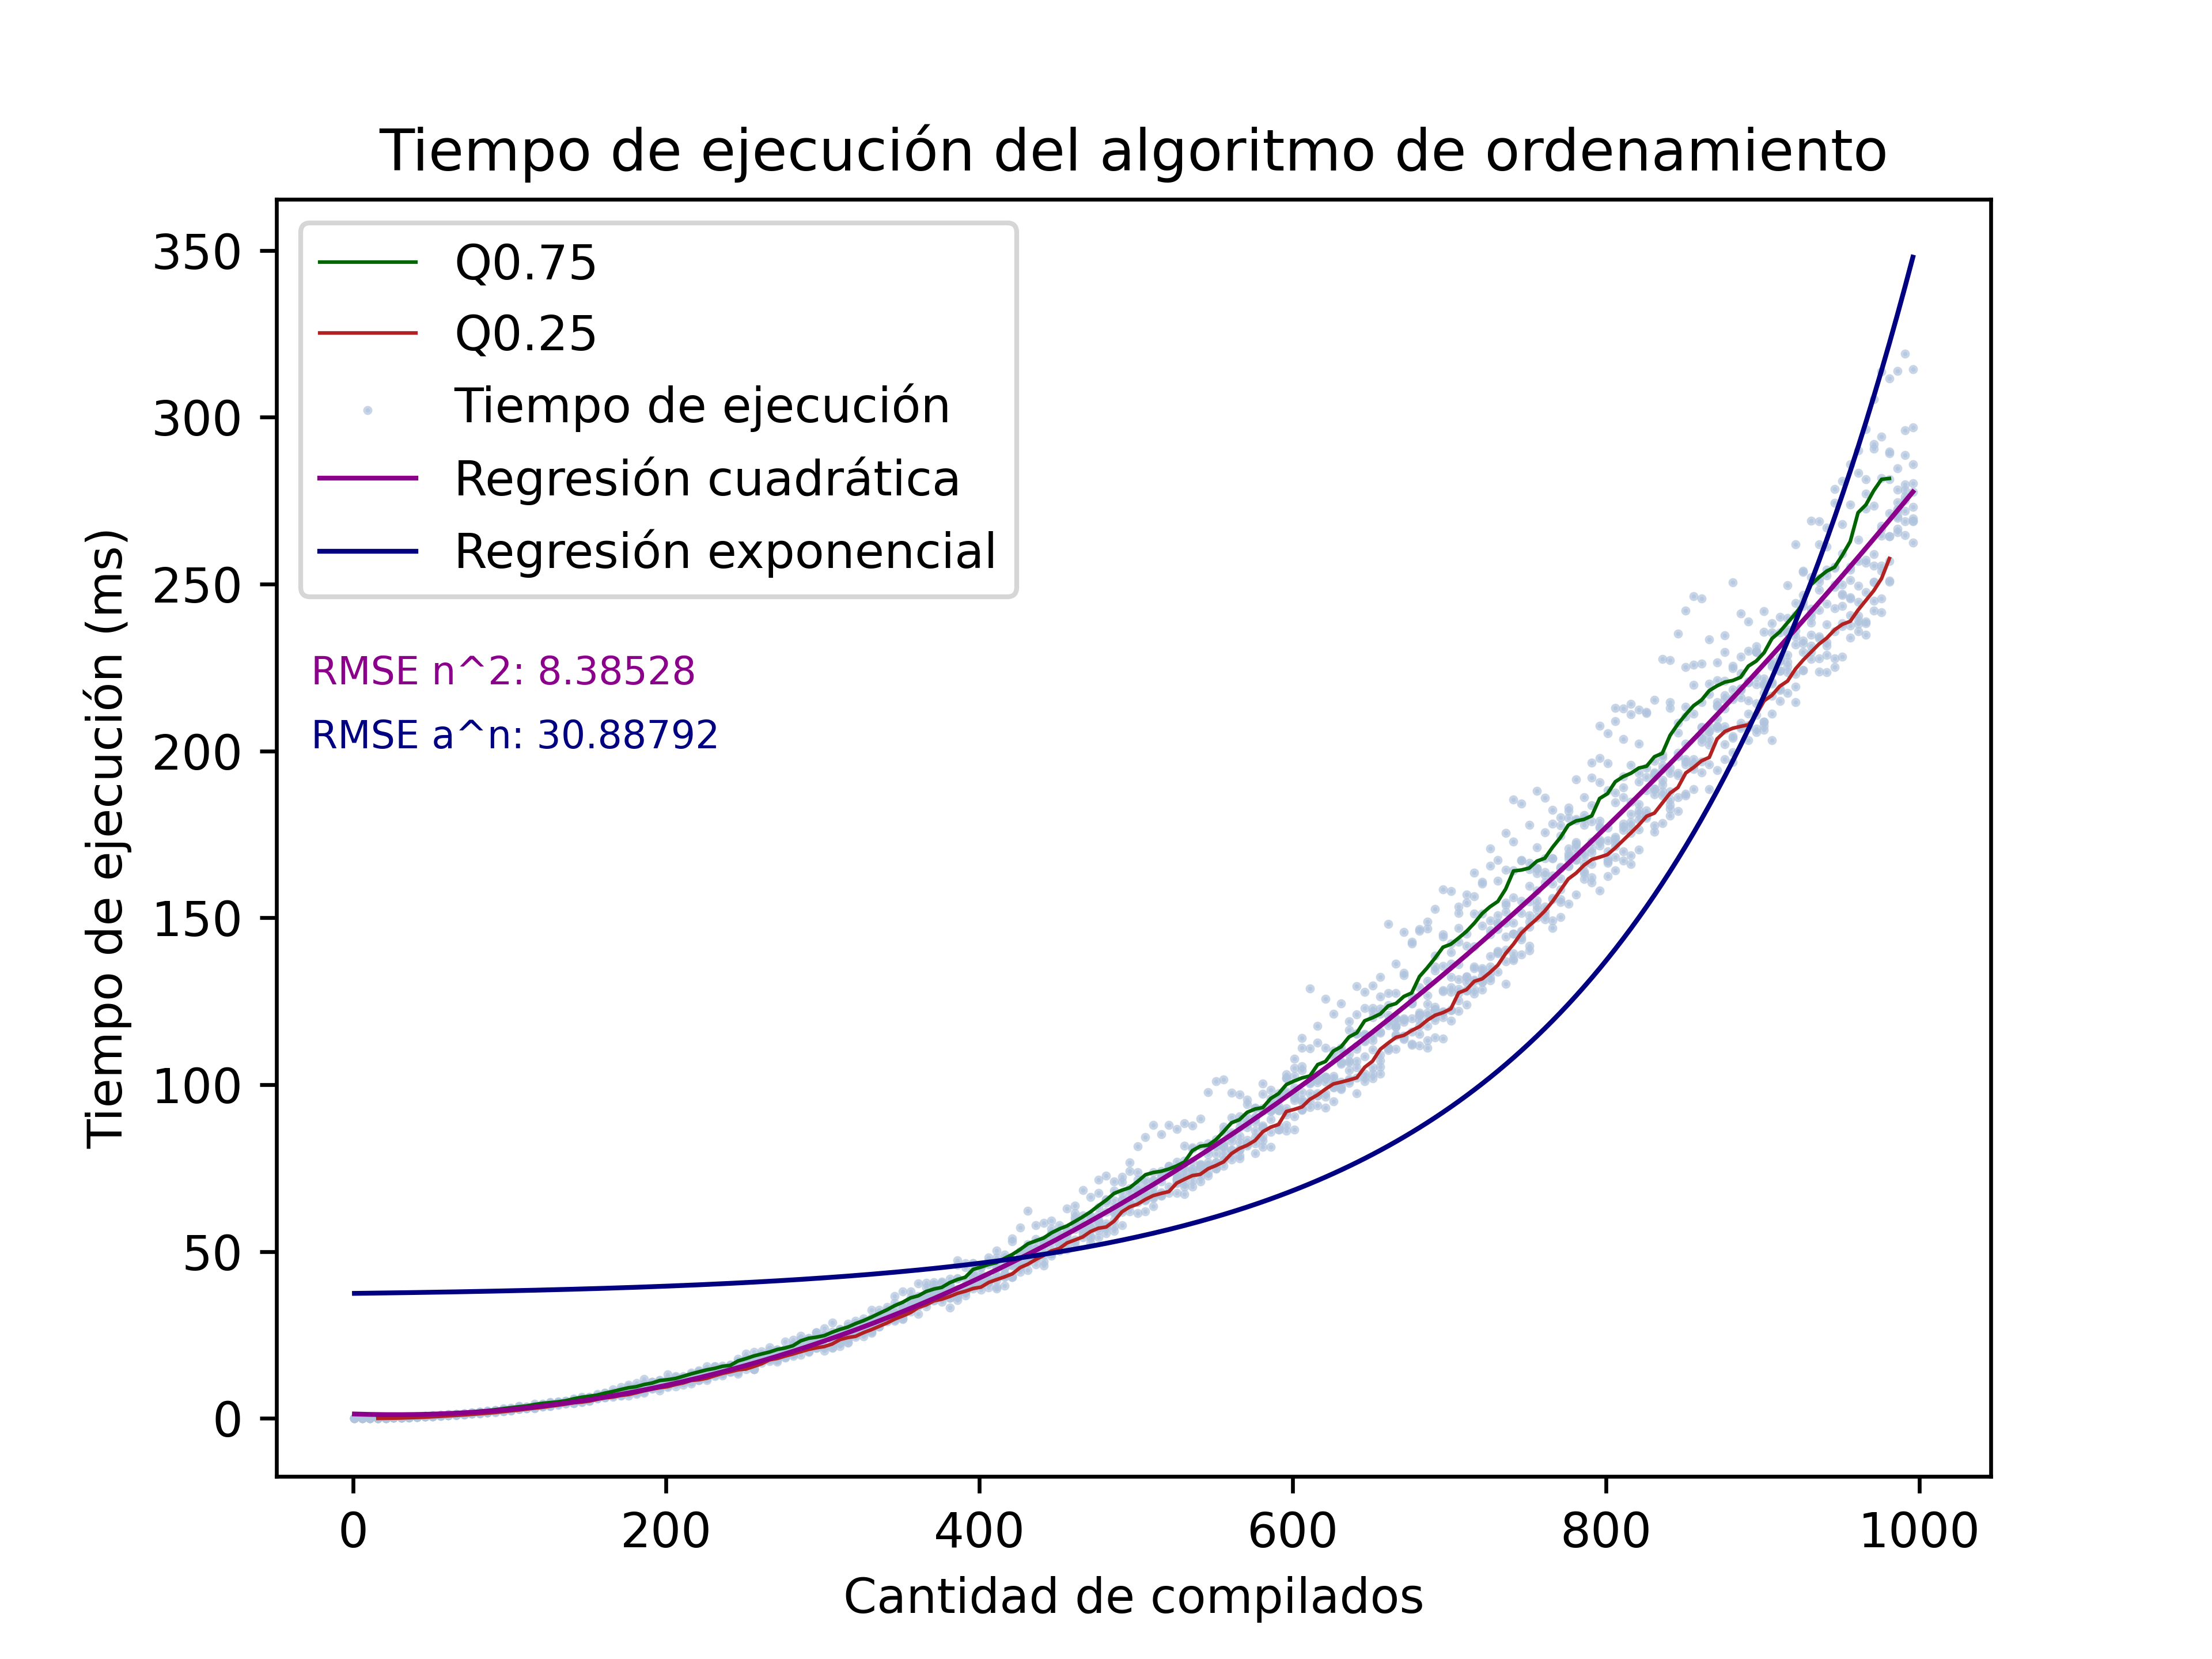
\includegraphics[width=0.8\textwidth]{img/tiempos_puntos.png}
    \caption{Tendencia de la complejidad algoritmica.}
    \label{fig:tiempos_puntos}
\end{figure}

De esta manera, mediante el gráfico y la validación a través del error cuadrático medio,
hemos comprobado que la curva cuadrática se adapta de manera más precisa a nuestros datos.

De esta forma pudimos comprobar empíricamente que la complejidad tiende a $\operatorname{O}(n^2)$.

Nótese que graficamos también dos curvas que demarcan una estimación de los cuantiles verticales $0.25$ y $0.75$. Esta estimación
se realizó calculando los cuantiles para un grupo pequeño centrado en cada punto. Estas curvas nos ayudan a dimensionar cómo la
varianza del tiempo de ordenamiento crece con el aumento del tamaño de la información de entrada.

Adicionalmente, graficamos la densidad de los tiempos que también brinda una visualización de cómo aumenta la varianza con el aumento del tamaño
de los datos de entrada. Ver figura \ref{fig:tiempos_densidad}. 

\begin{figure}[H]
    \centering
    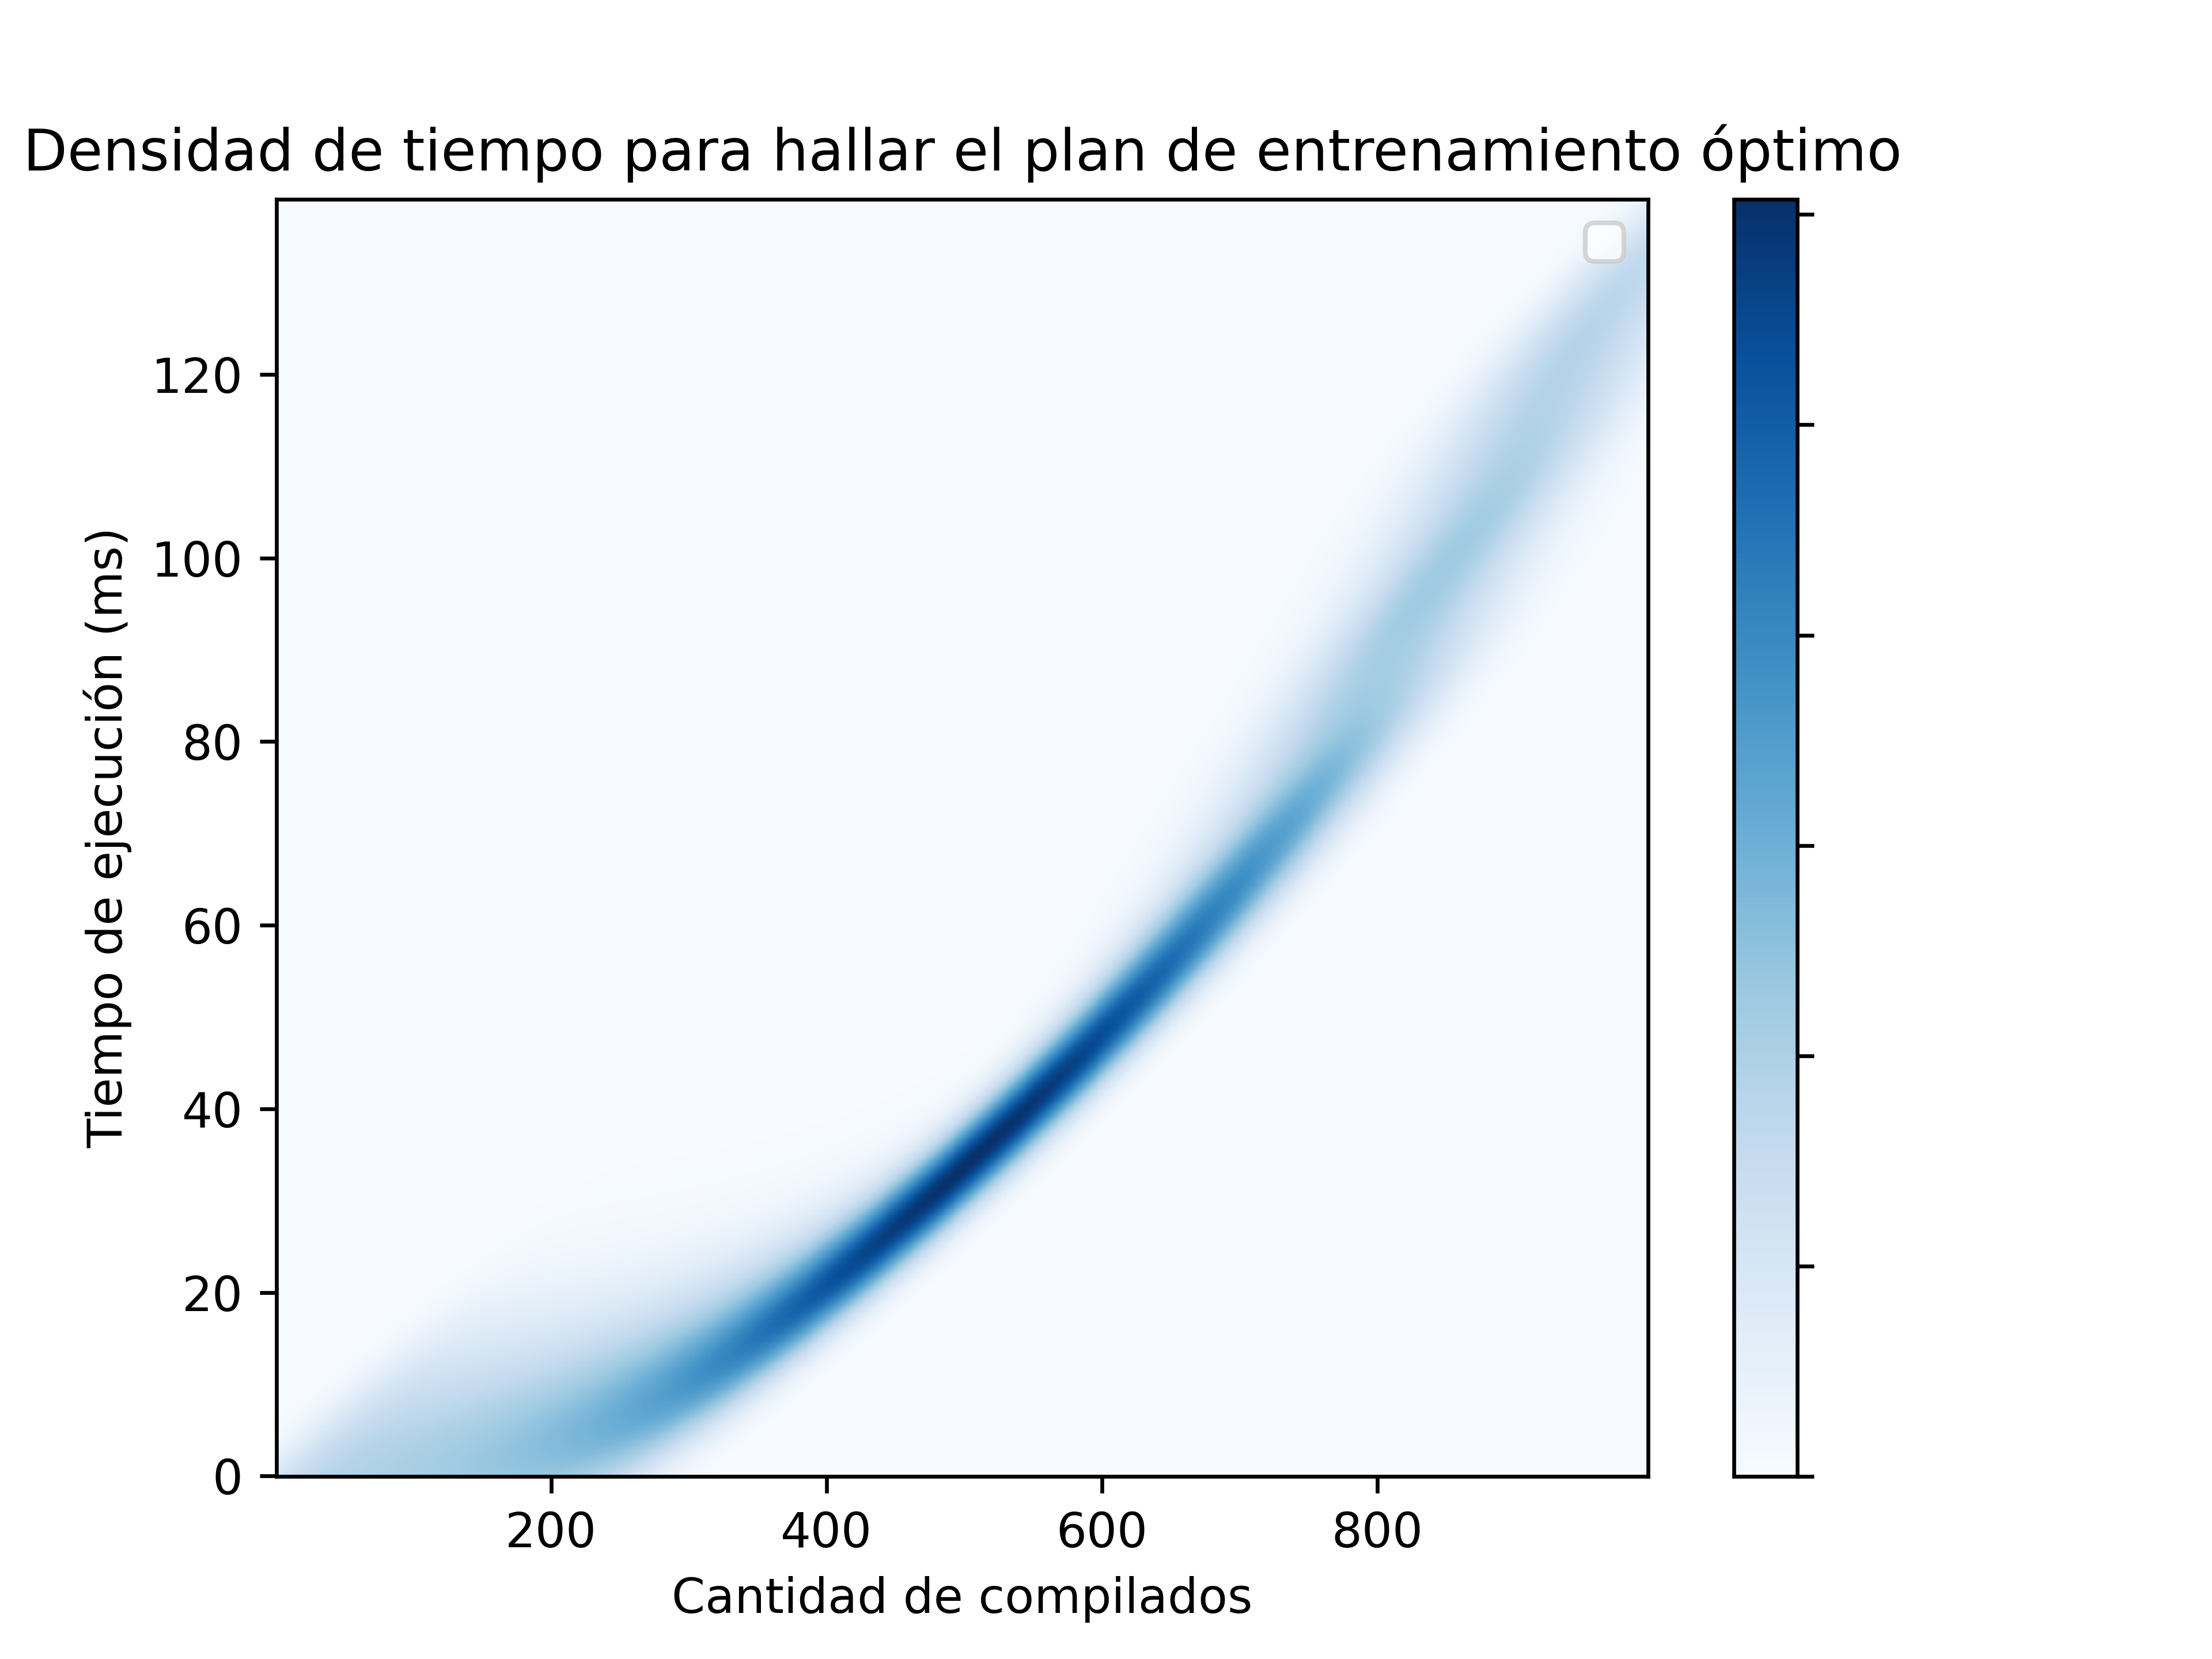
\includegraphics[width=0.8\textwidth]{img/tiempos_densidad.png}
    \caption{Densidad de mediciones.}
    \label{fig:tiempos_densidad}
\end{figure}
